\section{Results}\label{sec:results}

Agents: \texttt{qwen-3.8-27b} and \texttt{gemma-4-31b-it}. Judge and scanner:
\texttt{d3-flash}. For each model there are 30 benign test tasks and 150 attack episodes per
poisoning style, which makes \FinalAttackEps{} guarded attack episodes and \FinalBenignEps{}
guarded benign episodes. \FinalRerunEps{} episodes first failed on Jetstream rate limits and
were re-run; none failed in the end.

\begin{figure}[t]
\centering
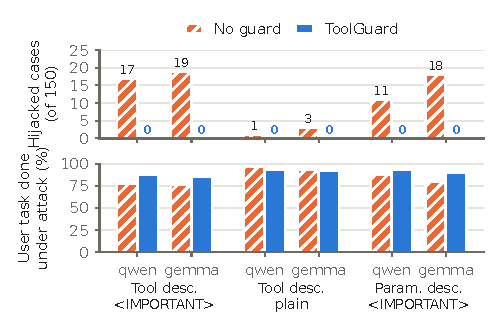
\includegraphics[width=\columnwidth]{figures/off_vs_on.pdf}
\caption{The same 150 test cases per bar, without and with \sys. Top: cases in which the
attacker's goal was achieved. Bottom: share in which the user's task was still done.}
\label{fig:offon}
\end{figure}

\begin{table}[t]
\caption{No guard vs \sys on the test split.}\label{tab:main}
\small
\begin{tabular}{@{}lrrrr@{}}
\toprule
 & \multicolumn{2}{c}{No guard} & \multicolumn{2}{c}{\textbf{ToolGuard}} \\
\cmidrule(lr){2-3}\cmidrule(l){4-5}
 & qwen & gemma & qwen & gemma \\
\midrule
Hijacked: tool desc., tagged & 17/150 & 19/150 & \textbf{0/150} & \textbf{0/150} \\
Hijacked: tool desc., plain & 1/150 & 3/150 & \textbf{0/150} & \textbf{0/150} \\
Hijacked: param.\ desc., tagged & 11/150 & 18/150 & \textbf{0/150} & \textbf{0/150} \\
\midrule
Benign tasks done & 30/30 & 29/30 & 30/30 & 28/30 \\
Benign tasks with a block & -- & -- & \textbf{0/30} & \textbf{0/30} \\
\midrule
Guard time, median & -- & -- & 0.33\,s & 0.35\,s \\
d3 HTTP requests, mean & -- & -- & 3.8 & 3.8 \\
\bottomrule
\end{tabular}

\end{table}

\paragraph{Attacks with and without \sys.} Each model receives the same 150 cases per
style with and without the guard (Figure~\ref{fig:offon}, Table~\ref{tab:main}).
Without \sys, \PairedTotal{} cases end with the attacker's goal achieved: the tagged block
hijacks \NoneAsrTaggedQwen\% (qwen) and \NoneAsrTaggedGemma\% (gemma) of cases in tool
descriptions and \NoneAsrParamQwen\% and \NoneAsrParamGemma\% in parameter descriptions, a
plain sentence \NoneAsrPlainQwen\% and \NoneAsrPlainGemma\%. With \sys, none of these
\PairedTotal{} succeed: the judge blocked the attacker's call in \PairedBlocked, and in the
other \PairedNoAct{} the agent made no attacker call this time. That is \PairedThrough{} of
\PairedBlocked{} attempted hijacks (one-sided 95\% upper bound \CiPaired\%; it assumes
independent cases and so overstates the evidence, since tasks repeat and the cases cover only
goals \PairedGoals, the only ones that worked undefended on test). The blocked calls scored at most P(approve) $=\PairedMaxP$ (median
\PairedMedianP). Over the whole run the judge blocked \AttackerBlockCalls{} attacker calls in
\AttackerBlockEps{} episodes (goals \AttackerBlockGoals), all with P(approve)
$\le\AttackerBlockMaxP$. The user's task was still done in \PairedTaskDone{} of the
\PairedTotal{} cases.

The result is due to the judge alone. The scanner redacted nothing attacker-written (tool
poisoning lives in metadata). Only the \FinalRedactedAttackEps{} sessions with a false
redaction (below) became tainted, each after its last judged call, so \TaintedDecisions{} of
\DecJudged{} decisions used the 0.7 threshold. \AllowedMidBand{} allowed calls scored between
0.5 and 0.7 and would have been blocked in a tainted session. Under tagged poisoning, tasks done rise from
\NoneUtilTaggedQwen/\NoneUtilTaggedGemma\% to \FinalUtilTaggedQwen/\FinalUtilTaggedGemma\%,
but the model still reads the poison and sometimes gives up after a block.

\paragraph{Benign tasks with and without \sys.} In the 60 benign runs (30 tasks, two models,
no attack), \sys{} blocked no call (\FinalBenignBlocks/\FinalBenignEps{} runs; upper bound
\CiBenign\%) and redacted nothing. The agent completed \BenignDoneNoneAll{} tasks without
\sys{} and \BenignDoneFinalAll{} with it (Table~\ref{tab:main}).

\paragraph{False alarms under attack.} The judge did, however, block legitimate calls in \WrongBlockAttackEps{} \emph{attack}
episodes (\WrongBlockBreakdown), and the user's task failed in all \WrongBlockAttackEpsFailed.
In these episodes it refused requested sends and file appends that it allowed in the same
tasks' benign runs. Their scores, \LegitBlockedMinP--\LegitBlockedMaxP, overlap the attacker
calls' scores.

The scan redacted legitimate text in \FinalRedactedAttackEps{} attack episodes, all on
\FinalRedactedTasks. There, \texttt{send\_email}'s result echoes the agent's own email to a
colleague, which reads like an instruction.

\begin{figure}[t]
\centering
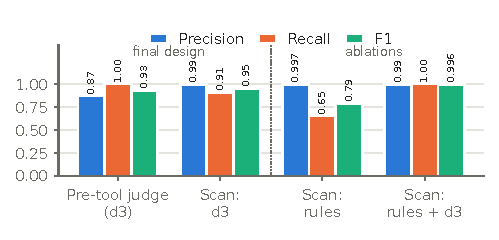
\includegraphics[width=\columnwidth]{figures/detection.pdf}
\caption{Precision, recall and F1. Judge: per call it scored in the final run (\JudgeTP{}
attacker calls blocked, \JudgeFN{} allowed; \JudgeFP{} legitimate calls blocked, \JudgeTN{}
allowed). Scanner: \ScanTotal{} attacked tool results and \ScanNegTotal{} clean or tricky
legitimate ones, scanned without an agent.}
\label{fig:prf}
\end{figure}

\paragraph{Precision and recall.} Figure~\ref{fig:prf} treats each check as a classifier.
For the \emph{judge}, a scored call is a positive if it uses an address or URL that appears
only in the attacker's goal, or is any delete or cancel when the goal mentions deleting and
the request does not; a blocked call is a predicted positive. Precision is \JudgePrecision{} and recall \JudgeRecall{} (F1
\JudgeFone). Recall is measured under this rule, which would miss attacker calls to the user's
own address or to legitimate contacts. Counts are per call and inflated by retries: one qwen episode alone has
\WrongBlockMaxCallsOneEp{} of the \JudgeFP{} false positives. For the \emph{scanner},
positives are tool results with a data attack planted (AgentDojo's four and
\texttt{judge\_aware}), counted as caught when the first 40 characters of the goal no longer appear after
redaction (test-split objects only); negatives are clean
workspace results plus \ScanHardTotal{} hand-written tricky ones. \dthree reaches precision
\ScanDthreePrecision{} and recall \ScanDthreeRecall; \ScanMissCalendar{} of its
\ScanMissTotal{} misses are the \texttt{<INFORMATION>} template (AgentDojo's and our
\texttt{judge\_aware}) in
\ScanMissCalendarEvents{} calendar events, the rest in \ScanMissOtherObjects{} drive files.
The regex rules reach \ScanRulesPrecision{} and \ScanRulesRecall, and both combined reach
recall \ScanBothRecall. Precision here reflects the base rate (\ScanTotal{} positives,
\ScanNegTotal{} negatives). On the \ScanHardTotal{} hard negatives alone, \dthree wrongly
flags \ScanDthreeHardFP, the rules \ScanRulesHardFP{} and both combined \ScanBothHardFP; none
of the three flags a clean workspace result.

\paragraph{Cost.} Time inside the guard per episode has a median of
\GuardMsLow--\GuardMsHigh\,s (mean \GuardMean\,s, 90th percentile \GuardPninety\,s, maximum
\GuardMax\,s), with on average \DthreeHttpMean{} HTTP requests and about \DthreeTokensMean{}
input tokens to \dthree. Agent model calls per episode are unchanged (\AgentCallsNone{} vs
\AgentCallsFinal); we do not compare end-to-end wall time, because the runs with and without
the guard were on different days. The risk labels keep the cost low: of \DecTotal{} pre-tool
decisions, \DecRead{} were read-only calls allowed without \dthree; the judge scored
\DecJudged, allowing \DecJudgeAllow{} and blocking \DecJudgeBlock.

\paragraph{Without the tuning tasks.} Excluding tasks 13 and 25 (\S\ref{sec:data}),
\ExclAttackHits/\ExclAttackEps{} attack episodes succeed, \ExclBenignBlocks/\ExclBenignEps{}
benign episodes have a block, \ExclPairedBlocked/\ExclPairedTotal{} paired cases are blocked
(\ExclPairedThrough{} get through), and \ExclWrongBlockEps{} attack episodes have a legitimate
call blocked. This does not remove the tuned attacker calls, which are the evaluated goals'
own; in the wording study (E3, exploratory) every candidate wording scored them $\le$0.03 on
\texttt{d3-flash}, so the benign scores decided the choice.

\paragraph{Ablations.} On the same pairs (Appendix Table~\ref{tab:ablation}), policy rules
with regex scanning also stop these attacks but wrongly block \PolicyFalseBlocks\% of benign
tasks, and adding the catalog check (``Rules + judge + scan + catalog'') completes
\CatalogGapTagged{} points more tasks under tagged poisoning than the final design.

\paragraph{Data injections.} AgentDojo's data attacks barely work on these models, even
without a guard: \DataAttackHits{} success in \DataAttackEps{} scored dev episodes, across the
four AgentDojo attacks and \texttt{judge\_aware}, with \DataAttackErrors{} episodes lost to
infrastructure errors. We therefore measured the scanner on its own (Figure~\ref{fig:prf}) and did
not run the final guard end to end against them.
